\documentclass[a4paper, 12pt, twoside, final, book, russian, fittopage, cyremdash, openright]{ncc}
\usepackage[T2A]{fontenc}
\usepackage[utf8]{inputenc}
\usepackage[russian]{babel}
\usepackage{extdash}
\usepackage{xspace}
\usepackage{ncccomma}
\usepackage{upgreek}
\usepackage{marvosym}
\usepackage{amsfonts}
\usepackage[font=small]{caption}
\usepackage{xfrac}
\usepackage{accents}
\usepackage{amsmath}
\renewcommand{\bfdefault}{b} % плотный жирный

\newcommand{\mcyr}[1]{\ensuremath{\text{\textit{#1}}}}
\newcommand{\cidx}[2]{\ensuremath{#1_{\mcyr{#2}}}}
\newcommand{\lkvl}{\ensuremath{\cidx{L}{КВЛ}}\xspace}
\newcommand{\bkvl}{\ensuremath{\cidx{B}{КВЛ}}\xspace}
\newcommand{\tsr}{\ensuremath{\cidx{T}{ср}}\xspace}
\newcommand{\ve}[1]{\ensuremath{\mathbf{#1}}\xspace}
\newcommand{\gammaV}{\ensuremath{\ve{\gamma V}}\xspace}
\newcommand{\vidx}[2]{\ensuremath{\cidx{\ve #1}{#2}}\xspace}
\newcommand{\gr}{\ensuremath{^\circ}\xspace}
\newcommand{\grC}{\ensuremath{^{\circ}C}\xspace}
\newcommand{\midelsign}{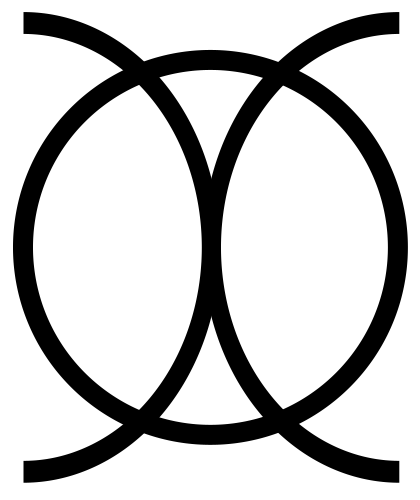
\includegraphics[width=1em]{midel_sign_vec.eps}\xspace}
\newcommand{\otdo}{--}
\newcommand{\motdo}{\==}
\newcommand{\ris}[1]{\ref{fig:#1}}
\newcommand{\rris}[1]{рис.~\ref{fig:#1}}
\newcommand{\Renum}{\ensuremath{\mathrm {Re}}}
\newcommand{\msq}{~м\ensuremath{^2}\xspace}
\newcommand{\gmsq}{~г/м$^2$\xspace}
\newcommand{\kgmsq}{~кг/м$^2$\xspace}
\newcommand{\speedms}{~м$/$с\xspace}
\newcommand{\coursespelengs}[1]{\ensuremath{\text{\textit{#1}}}\xspace}
\newcommand{\IK}{\coursespelengs{ИК}}
\newcommand{\IP}{\coursespelengs{ИП}}
\newcommand{\OIP}{\coursespelengs{ОИП}}
\newcommand{\KU}{\coursespelengs{КУ}}
\newcommand{\MK}{\coursespelengs{МК}}
\newcommand{\OP}{\coursespelengs{ОП}}
\newcommand{\OMP}{\coursespelengs{ОМП}}
\newcommand{\Klb}{\ensuremath{\text{\textit{К}}_{\text{\textit{лев.борта}}}}\xspace}
\newcommand{\Kpb}{\ensuremath{\text{\textit{К}}_{\text{\textit{пр.борта}}}}\xspace}
\newcommand{\KK}{\coursespelengs{КК}}
\newcommand{\KP}{\coursespelengs{КП}}
\newcommand{\OKP}{\coursespelengs{ОКП}}
\newcommand{\MP}{\coursespelengs{МП}}
\newcommand{\PU}{\mcyr{ПУ}\xspace}
\newcommand{\PUb}{\ensuremath{\mcyr{ПУ}_\beta}\xspace}
\newcommand{\AP}{\cidx{A}{П}\xspace}
\newcommand{\Ost}{\ensuremath{{O^{st}}}\xspace}
\newcommand{\tauAries}{\ensuremath{\uptau^{\text{\Aries}}}\xspace}
\newcommand{\tAries}{\ensuremath{t^{\text{\Aries}}}\xspace}
\newcommand{\tday}{\ensuremath{^\text{д}}\xspace}
\newcommand{\tmin}{\ensuremath{^\text{м}}\xspace}
\newcommand{\thr}{\ensuremath{^\text{ч}}\xspace}
\newcommand{\tsec}{\ensuremath{^\text{с}}\xspace}
\newcommand{\SunPower}{\ensuremath{^\text{\Sun}}}
\newcommand{\TSun}{\ensuremath{T^{\text{\Sun}}}}
\newcommand{\tSun}{\ensuremath{t^{\text{\Sun}}}}
\newcommand{\TNo}{\ensuremath{T_{\text{\No}}}\xspace}
\newcommand{\NoC} {\cidx{\No}{C}\xspace}
\newcommand{\mathNo}{\text{\No}}
\newcommand{\hhmm}[2]{\ensuremath{#1\thr~#2\tmin}}
\newcommand{\hhmmss}[3]{\ensuremath{#1\thr~#2\tmin~#3\tsec}}
\newcommand{\Tgr}{\cidx{T}{гр}\xspace}
\newcommand{\tGR}{\cidx{t}{гр}\xspace}
\newcommand{\ppp}{\ensuremath{\text{п.}}}
\newcommand{\grmm}[2]{\ensuremath{#1\gr\,#2'}}
\newcommand{\grmmr}[3]{\ensuremath{\grmm{#1}{#2}\,#3}}
\newcommand{\grmmss}[3]{\ensuremath{#1\gr\,#2'\,#3''}}
\newcommand{\starName}[1]{\scalebox{1.5}{\raisebox{-0.2ex}{$\ast$}}#1}
\newcommand{\starSign}{\scalebox{1.5}{\raisebox{-0.2ex}{\ast}}}
\newcommand{\SunriseA}{\ensuremath{{\widehat{\text{\Sun}}}}\xspace}
\newcommand{\Sunset} {\ensuremath{{\uwidehat{\text{\Sun}}}}\xspace}
\newcommand\bigfrac[2]{\frac{\displaystyle #1}{\displaystyle #2}}

\newcommand{\alphaStar}[1]{$\upalpha$~#1}
\newcommand{\deltaStar}[1]{$\updelta$~#1}
\newcommand{\epsilonStar}[1]{$\varepsilon$~#1}
\newcommand{\gammaStar}[1]{$\upgamma$~#1}
\newcommand{\etaStar}[1]{$\upeta$~#1}
\newcommand{\betaStar}[1]{$\upbeta$~#1}

\newcommand{\taustar}{\ensuremath{\uptau^*}\xspace}

\newcommand{\p}[1]{\noindent\textbf{#1.}\label{par:#1}}
\newcommand{\lp}[1]{#1~\pageref{par:#1}}

\newcommand*{\appnav}[2][4]{\ref{app:#1}~\textit{#2}}

\newcommand{\uhat}{\underaccent{\check}}

\newcommand{\uwidehat}[1]{%
  \mathpalette\douwidehat{#1}%
}

%\newcommand\groupequation[2][17pt]{%
%  \setbox0=\hbox{$\displaystyle#2$}%
%  \stackengine{0pt}{\copy0}{%
%    \makebox[\linewidth]{\hfill$\left.\rule{0pt}{\ht0}\right\}$\kern#1}}
%  {O}{c}{F}{T}{L}
%}
  
\makeatletter
\newcommand{\douwidehat}[2]{%
  \sbox0{$\m@th#1\widehat{\hphantom{#2}}$}%
  \sbox2{$\m@th#1x$}
  \sbox4{$\m@th#1#2$}
  \dimen0=\ht0
  \advance\dimen0 -.8\ht2
  \dimen2=\dp4
  \rlap{%
    \raisebox{\dimexpr\dimen0-\dimen2}{%
      \scalebox{1}[-1]{\box0}%
    }%
  }%
  {#2}%
}
\makeatother
